\documentclass[twocolumn]{article}
% Graphics with TikZ
\usepackage{tikz}
% Enable TikZ libraries used by figures (coordinate calc for positioned nodes, arrows.meta for arrowheads)
\usetikzlibrary{calc,arrows.meta}

\title{A Proposal For A Bit-operations based Neural Network architecture\thanks{To Bénédicte Brion}}
\author{Bernhard Gerlach  \\
	Private Research Lab  \\
	\and 
	The Other Dude \\
	His Company / University \\
	}

\date{\today}

% Hint: \title{what ever}, \author{who care} and \date{when ever} could stand 
% before or after the \begin{document} command 
% BUT the \maketitle command MUST come AFTER the \begin{document} command! 
\begin{document}

\maketitle

\begin{abstract}
Short introduction to subject of the paper \ldots 
\end{abstract}

\section{Introduction}
Make it possible for all to write documents with \LaTeX{}!

\paragraph{Outline}
First we start with a little example of the article class, which is an 
important documentclass. 


\section{Related Work}\label{sec:related}
% TODO: Summarise prior art and position the contribution relative to existing architectures and methods.

\section{Background and Preliminaries}\label{sec:background}
% TODO: Define notation, basic concepts, and any baseline models needed for understanding.

Current neuronal network architectures predominantly rely on matrix multiplications to process and transform data. This section provides an overview of the fundamental concepts and notations that underpin traditional neural networks, as well as the preliminaries necessary for understanding the proposed bit-level operations.

\subsection{Notation}
We denote vectors in bold lowercase (e.g., \(\mathbf{x}\)) and matrices in bold uppercase (e.g., \(\mathbf{W}\)). The \(i\)-th element of a vector \(\mathbf{x}\) is denoted as \(x_i\), and the element in the \(i\)-th row and \(j\)-th column of a matrix \(\mathbf{W}\) is denoted as \(W_{ij}\).

\subsection{Basic Concepts}
Neural networks consist of layers of interconnected nodes (neurons), where each connection is associated with a weight. The output of each neuron is computed as a weighted sum of its inputs, followed by a non-linear activation function. Formally, for a single neuron, the output \(y\) can be expressed as:
\[
y = f\left(\sum_{i} W_{i} x_{i} + b\right)
\]
where \(f\) is the activation function and \(b\) is the bias term.

\subsection{Baseline Models}
The most common baseline model for comparison in this paper is the fully connected feedforward neural network (FNN), which consists of multiple layers of neurons with dense connections. Other relevant models include convolutional neural networks (CNNs) for image processing tasks and recurrent neural networks (RNNs) for sequential data.


\section{Proposed Method}\label{sec:method}
% TODO: Present the new neuronal-network concept, intuition, formal definition and key equations.


% Example visualization: three rows of 8-bit sequences (MSB/LSB labeled) drawn with TikZ to illustrate the proposed encoding/neuronal input layout.
\begin{center}
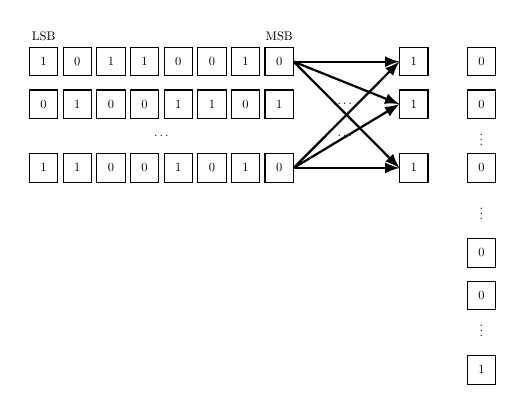
\begin{tikzpicture}[scale=0.45,transform shape, box/.style={draw, minimum size=8mm, inner sep=1pt}, node distance=0.9cm]
    % sequence can be changed; this is a small "random" example
    \foreach \i [count=\xi from 0] in {1,0,1,1,0,0,1,0} {
        \node[box] (n\xi) at (\xi*0.95,0) {\i};
    }

    % labels above leftmost and rightmost boxes
    \node[above=2pt] at (n0.north) {LSB};
    \node[above=2pt] at (n7.north) {MSB};

    % add an extra box after a horizontal gap equal to 3 box widths
    % compute a random 0/1 for the extra box on the first row
    \pgfmathtruncatemacro{\rnda}{random(0,1)}
    \node[box] (nextra) at (11*0.95,0) {\rnda};

    % second row (random 0/1 sequence)
    \foreach \i [count=\xi from 0] in {0,1,0,0,1,1,0,1} {
        \node[box] (m\xi) at (\xi*0.95,-1.2) {\i};
    }
    % extra box after a gap of 3 boxes on the second row
    \pgfmathtruncatemacro{\rndb}{random(0,1)}
    \node[box] (mextra) at (11*0.95,-1.2) {\rndb};

    % three small dots between the last box (m7) and the extra rightmost box on the second row
    \node at (8.5,-1.2) {$\ldots$};
    \node at (8.5,-2.1) {$\ldots$};

    % centered triple dot between rows
    \node at (3.325,-2.1) {$\ldots$};

    % third row (another random 0/1 sequence)
    \foreach \i [count=\xi from 0] in {1,1,0,0,1,0,1,0} {
        \node[box] (p\xi) at (\xi*0.95,-3.0) {\i};
    }
    % extra box after a gap of 3 boxes on the third row
    \pgfmathtruncatemacro{\rndc}{random(0,1)}
    \node[box] (pextra) at (11*0.95,-3.0) {\rndc};

    % right-side vertical column (single column), placed relative to the extra box so it's visible
    \coordinate (colx) at ($(nextra.east)+(1.5,0)$);
    \pgfmathtruncatemacro{\colA}{random(0,1)}
    \node[box] (col1) at ($(colx)+(0,0)$) {\colA};
    \pgfmathtruncatemacro{\colB}{random(0,1)}
    \node[box] (col2) at ($(colx)+(0,-1.2)$) {\colB};
    % vertical dots indicating omitted rows
    \node at ($(colx)+(0,-2.1)$) {$\vdots$};
    \pgfmathtruncatemacro{\colC}{random(0,1)}
    \node[box] (col3) at ($(colx)+(0,-3.0)$) {\colC};
    % small vertical gap then more omitted rows
    \node at ($(colx)+(0,-4.2)$) {$\vdots$};
    \pgfmathtruncatemacro{\colD}{random(0,1)}
    \node[box] (col4) at ($(colx)+(0,-5.4)$) {\colD};
    \pgfmathtruncatemacro{\colE}{random(0,1)}
    \node[box] (col5) at ($(colx)+(0,-6.6)$) {\colE};
    \node at ($(colx)+(0,-7.5)$) {$\vdots$};
    \pgfmathtruncatemacro{\colF}{random(0,1)}
    \node[box] (col6) at ($(colx)+(0,-8.7)$) {\colF};

    % arrows from the first-row rightmost box (n7) to each of the extra rightmost boxes
    \draw[->,thick,>=latex] (n7.east) -- (nextra.west);
    \draw[->,thick,>=latex] (n7.east) -- (mextra.west);
    \draw[->,thick,>=latex] (n7.east) -- (pextra.west);
    % arrows from the second-row rightmost box (m7) to each of the extra rightmost boxes
    \draw[->,thick,>=latex] (p7.east) -- (nextra.west);
    \draw[->,thick,>=latex] (p7.east) -- (mextra.west);
    \draw[->,thick,>=latex] (p7.east) -- (pextra.west);
\end{tikzpicture}
\end{center}


\section{Implementation Details}\label{sec:implementation}
% TODO: Provide architecture specifics, training regimen, datasets, reproducibility notes and environment.

\section{Experimental Setup}\label{sec:experiments}
% TODO: Describe tasks/benchmarks, baselines, ablations and evaluation metrics.

\section{Results}\label{sec:results}
% TODO: Add quantitative tables, statistical analysis and efficiency measurements.

\section{Qualitative Analysis}\label{sec:qualitative}
% TODO: Include visualisations, failure cases and interpretability insights.

\section{Discussion}\label{sec:discussion}
% TODO: Analyse why the method works, its limitations and applicability.

\section{Conclusions}\label{conclusions}
There is no longer \LaTeX{} example which was written by \cite{doe}.

\section*{Acknowledgements}\label{sec:ack}
% TODO: Acknowledge funding, contributors, and dataset licenses.

\appendix
\section{Appendix: Additional Details}\label{sec:appendix}
% TODO: Extended hyperparameters, proofs, and extra experiments.

\begin{thebibliography}{9}
\bibitem[Doe]{doe} \emph{First and last \LaTeX{} example.},
John Doe 50 B.C. 
\end{thebibliography}

\end{document}
